% Set up document

\documentclass[xcolor={usenames,dvipsnames}]{beamer}
\usetheme{Madrid}
\setbeamersize{text margin left=5mm,text margin right=5mm}

% Dark background with non-white words: 
% \usecolortheme{owl}
% \setbeamercolor{normal text}{fg=yellow}
% \setbeamercolor{frametitle}{fg=yellow}
% \usebeamercolor[fg]{normal text}

% Used to create a section slide between section
\AtBeginSection[]{
  \begin{frame}[noframenumbering, plain]
  \vfill
  \centering
  \begin{beamercolorbox}[sep=8pt,center,shadow=true,rounded=true]{title}
    \usebeamerfont{title}\insertsectionhead\par%
  \end{beamercolorbox}
  \vfill
  \end{frame}
}

% Used to create a subsection slide between subsections
% \AtBeginSubsubsection{\frame{\subsubsectionpage}}
\AtBeginSubsection[]{
  \begin{frame}[noframenumbering, plain]
  \vfill
  \centering
  \begin{beamercolorbox}[sep=8pt,center,shadow=true,rounded=true]{title}
    \usebeamerfont{title}\insertsectionhead:\par\phantom{space please}\par\insertsubsectionhead\par%
  \end{beamercolorbox}
  \vfill
  \end{frame}
}


% Remove default navigation symbols and add just  page number
\setbeamertemplate{navigation symbols}{} % Clear default navigation
% \addtobeamertemplate{navigation symbols}{}{%
%     \usebeamerfont{footline}%
%     \usebeamercolor[fg]{footline}%
%     \hspace{1em}%
%     \insertframenumber/\inserttotalframenumber
% }

% Remove from footer the names, institution, date...
% and just leave page number:
\setbeamertemplate{footline}[frame number]


% For manual font size:
\usepackage{anyfontsize}

% For smaller URLs:
\newcommand{\smallurl}[1]{\textcolor{blue}{\fontsize{4pt}{4.8pt}\selectfont \url{#1}}}
%%%%%%%%%%%%%%%%%%%%%%%%%%%%%%%%%%%%%%%%%%%%%%%%%%%%%%%%%%%%%%%

%%%%%%%%%%%%%%%%%%%%%%%%%%%%%%%%%%%%%%%%%%%%%%%%%%%%%%%%%%%%%%%

% Title page

\title{Stroke Audit Machine Learning (SAMueL) \\ Advisory Group November 2022}
\subtitle{Investigating variation in thrombolysis use with clinical pathway simulation and explainable AI}


%\institute{Overleaf}
\date{November 2022}


\begin{document}

%\frame{\titlepage}

\begin{frame}
\titlepage

\end{frame}


%%%%%%%%%%%%%%%%%%%%%%%%%%%%%%%%%%%%%%%%%%%%%%%%%%%%%%%%%%%%%%%

\begin{frame}
\frametitle{Outline}
\tableofcontents
\end{frame}

%%%%%%%%%%%%%%%%%%%%%%%%%%%%%%%%%%%%%%%%%%%%%%%%%%%%%%%%%%%%%%%
\section{Modelled stroke pathway}

%%%%%%%%%%%%%%%%%%%%%%%%%%%%%%%%%%%%%%%%%%%%%%%%%%%%%%%%%%%%%%%

\begin{frame}
\frametitle{Breaking down the emergency stroke pathway into key steps}
\begin{center}
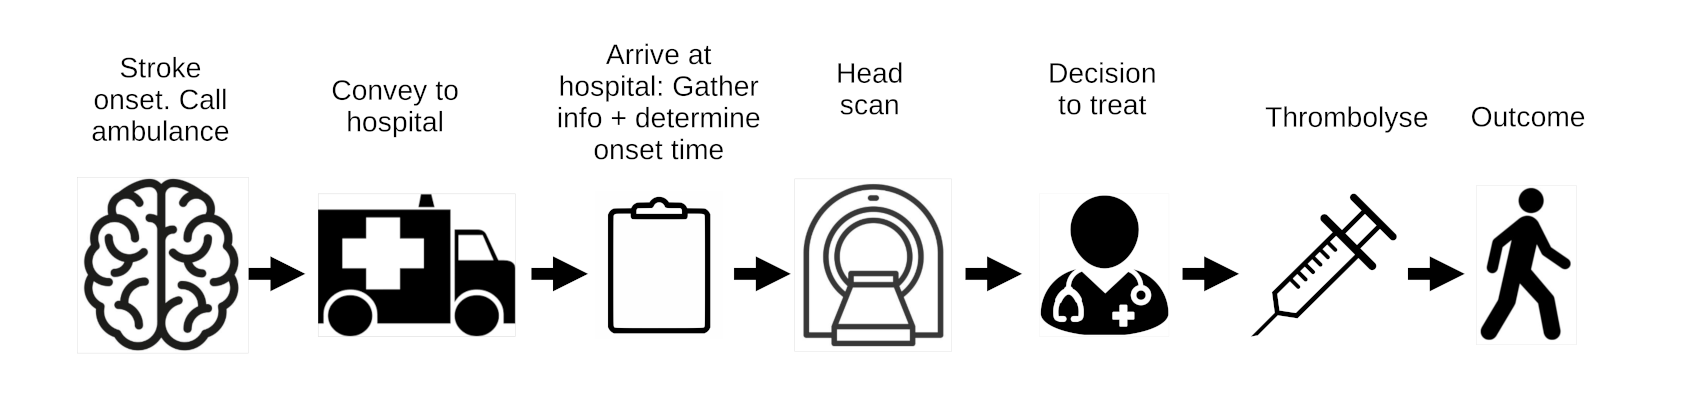
\includegraphics[width=1.0\textwidth]{./images/pathway}
\end{center}
We can model key changes to pathway:
\begin{small}
\begin{itemize}
    \item What if the pathway were faster?
    \item What if hospital determined the stroke onset time in more patients?
    \item What if clinical decision-making was like that of \emph{benchmark} hospitals? (Predict what treatment a patient would receive at other hospitals).
\end{itemize}
\end{small}
\footnotesize{We model these changes with a hospital's own patient population, to allow for inter-hospital variation in patient population characteristics.}
\end{frame}

%%%%%%%%%%%%%%%%%%%%%%%%%%%%%%%%%%%%%%%%%%%%%%%%%%%%%%%%%%%%%%%
\section{SAMueL-1 summary}


%%%%%%%%%%%%%%%%%%%%%%%%%%%%%%%%%%%%%%%%%%%%%%%%%%%%%%%%%%%%%%%

\begin{frame}
\frametitle{SAMueL-1 Summary: What is the problem?}
\begin{center}
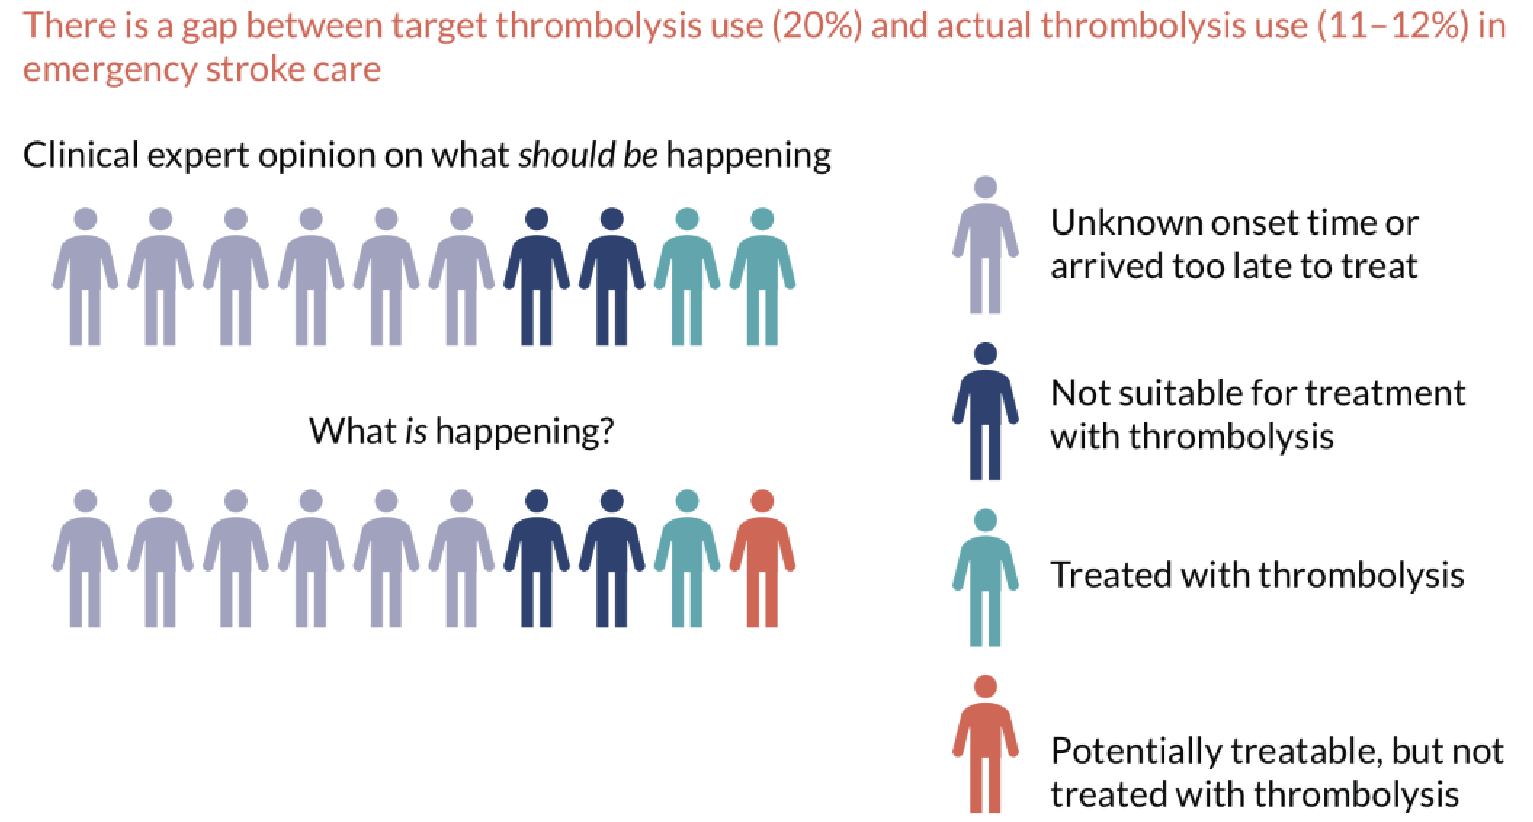
\includegraphics[width=1.0\textwidth]{./images/sam_summary_pt_1}
\end{center}
\end{frame}

\begin{frame}
\frametitle{SAMueL-1 Summary: What did we test?}

We used clinical pathway simulation and machine learning to analyse a series of \emph{what if?} questions:

\begin{itemize}
    \setlength\itemsep{3mm}
    \item What if arrival-to-treatment time was 30 minutes?
    \item what if all hospitals determined stroke onset time as frequently as an \emph{upper quartile} hospital (a hospital ranked 25 out of 100, for determining stroke onset time).
    \item What if decisions to thrombolyse were made according to a majority vote of 30 benchmark hospitals?
\end{itemize}

For each hospital we use their own patients to ask these questions, to allow for differences in local patient populations.
\end{frame}

\begin{frame}
\frametitle{SAMueL-1 Summary: What did we find?}
\begin{center}
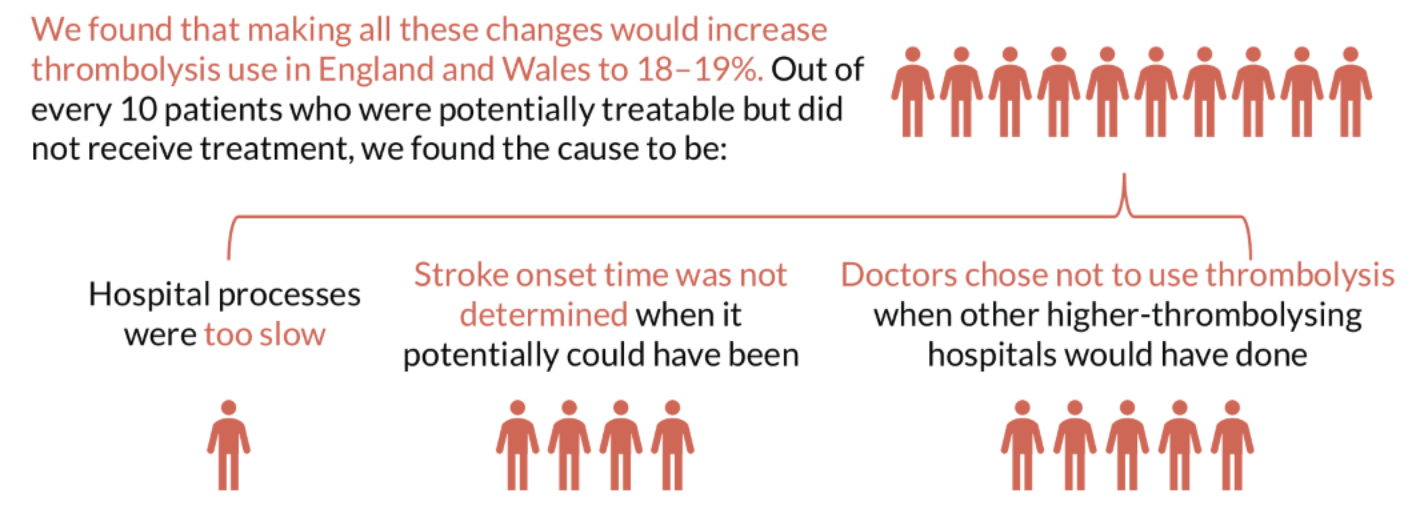
\includegraphics[width=1.0\textwidth]{./images/sam_summary_pt_3}
\end{center}
\end{frame}

%%%%%%%%%%%%%%%%%%%%%%%%%%%%%%%%%%%%%%%%%%%%%%%%%%%%%%%%%%%%%%%

\begin{frame}
\frametitle{Applying our models at hospital level}

\begin{center}
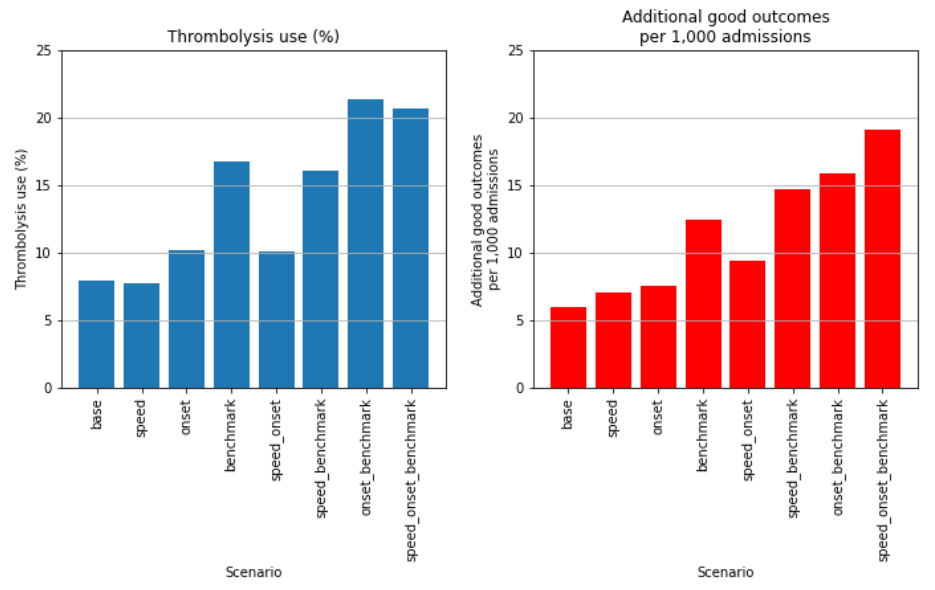
\includegraphics[width=0.95\textwidth]{./images/hosp_scenario_1}
\end{center}

\end{frame}

%%%%%%%%%%%%%%%%%%%%%%%%%%%%%%%%%%%%%%%%%%%%%%%%%%%%%%%%%%%%%%%
\section{Machine learning - learning and comparing decisions to thrombolyse between hopsitals}


%%%%%%%%%%%%%%%%%%%%%%%%%%%%%%%%%%%%%%%%%%%%%%%%%%%%%%%%%%%%%%%

\begin{frame}
\frametitle{Machine learning overview}
\begin{center}
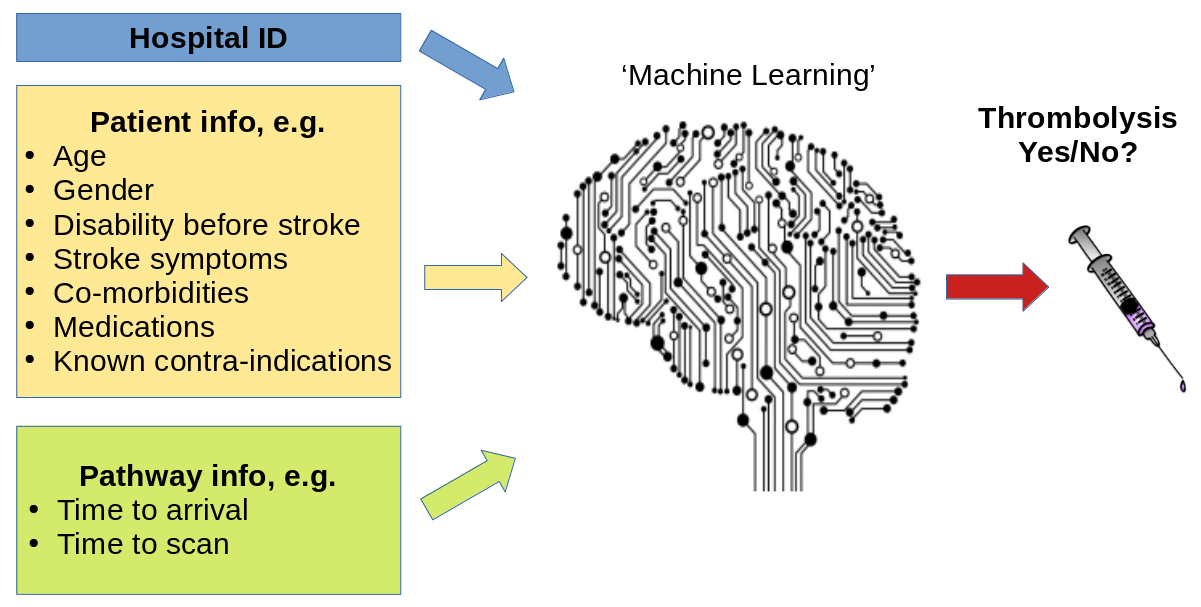
\includegraphics[width=0.90\textwidth]{./images/ml_model_high_level}
\end{center}


Machine learning (and nearly all \emph{artificial intelligence}) is based on the simple principle of recognising similarity to what has been seen before.
\vspace{3mm}

We accessed 240,000 emergency stroke admissions in England and Wales over three years.
\end{frame}

%%%%%%%%%%%%%%%%%%%%%%%%%%%%%%%%%%%%%%%%%%%%%%%%%%%%%%%%%%%%%%%

\begin{frame}{Model accuracy, and simplification}

Our machine learning models use XGBoost classification, and are based on all patients who arrive within 4 hours of known stroke onset.

\vspace{5mm}

\begin{columns}[T] % [T] Top aligns columns

    \begin{column}{0.5\textwidth}
    
        The full model has 61 patient features:
        
        \begin{footnotesize}
        \begin{itemize}
            \item Overall accuracy = 85.2\%
            \item Best combined sensitivity and specificity = 84.3\%
            \item ROC AUC = 0.921
        \end{itemize}
        \end{footnotesize}
        
        \vspace{3mm}
        
        A simplified model with 8 features
        
        \begin{footnotesize}
        \begin{itemize}
            \item Overall accuracy = 84.8\%
            \item Best combined sensitivity and specificity = 83.8\%
            \item ROC AUC = 0.916
        \end{itemize}
        \end{footnotesize}
    \end{column}
    
    \begin{column}{0.5\textwidth}
    The 8 features of the simplified model are:
        \begin{footnotesize}
        \begin{enumerate}
            \item Arrival-to-scan time
            \item Stroke type (infarction/haemorrhage)
            \item Stroke severity (NIHSS)
            \item Precise or estimated stroke onset time
            \item Prior disability level (mRS)
            \item Stroke team
            \item Use of AF anticoagulants
            \item Onset-to-arrival time
        \end{enumerate}
        \end{footnotesize}
        
    \vspace{2mm}
    \tiny{There are only very weak correlations between the selected features with no R-squared being greater than 0.05.}
    \end{column}
    
\end{columns}
\end{frame}


%%%%%%%%%%%%%%%%%%%%%%%%%%%%%%%%%%%%%%%%%%%%%%%%%%%%%%%%%%%%%%%

\begin{frame}
\frametitle{Explaining model predictions with SHAP values}

SHAP values show the influence of features (even for \emph{`black box'} models).

\begin{center}
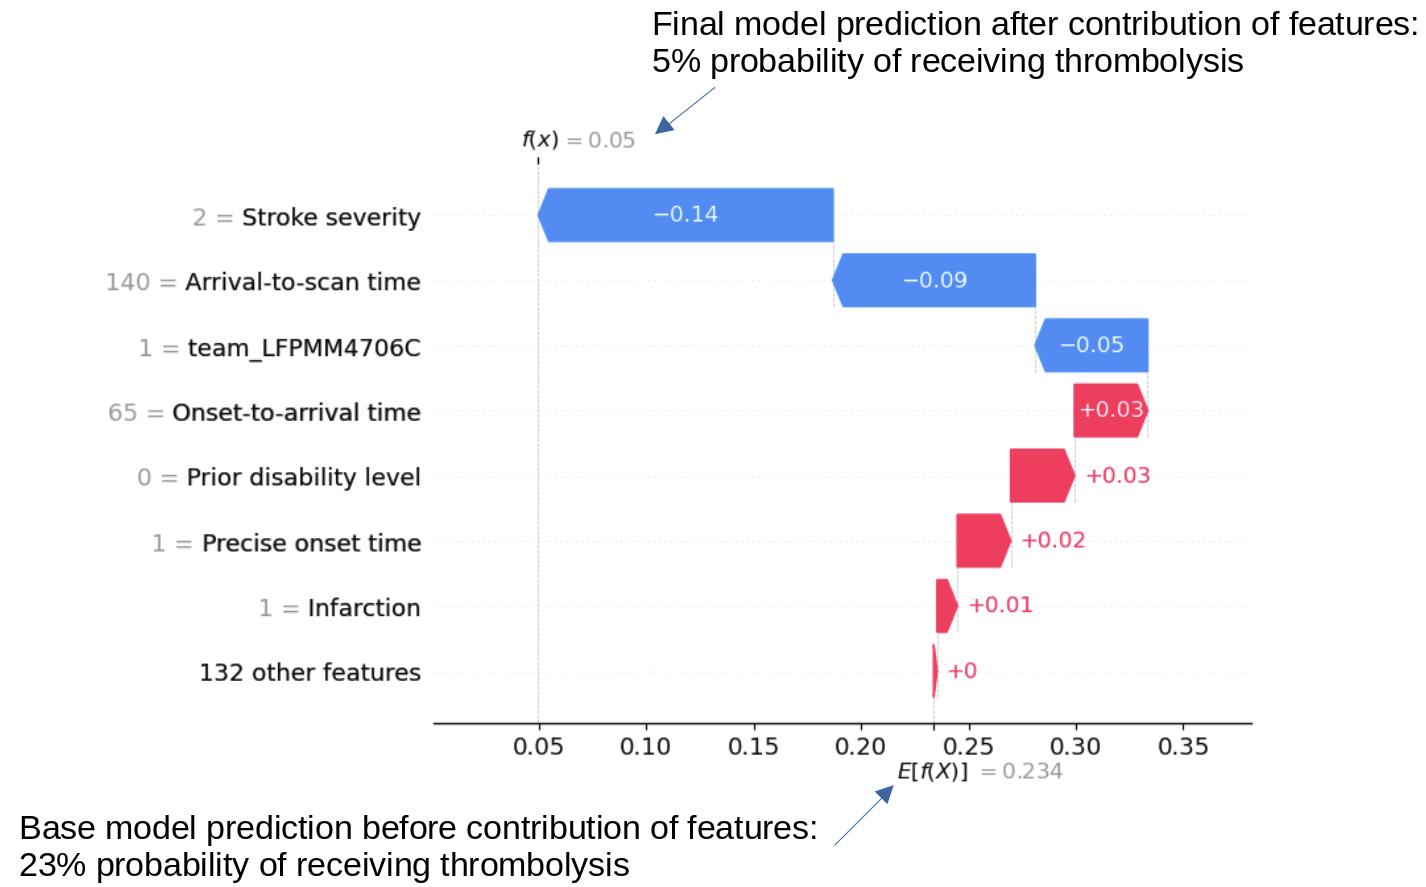
\includegraphics[width=0.85\textwidth]{./images/xgb_waterfall_low_probability.jpg}
\end{center}
\footnotesize
Note: The effect of team ID can depend on other patient characteristics.
\end{frame}

%%%%%%%%%%%%%%%%%%%%%%%%%%%%%%%%%%%%%%%%%%%%%%%%%%%%%%%%%%%%%%%

\begin{frame}
\frametitle{What drives use of thrombolysis across all hospitals?}

\footnotesize{Note: SHAP values here are \emph{log odds}. Each step-change in value of \textpm 1 changes the chances of receiving thrombolysis about 3-fold. (Plots are in order of feature importance.)}

\begin{center}
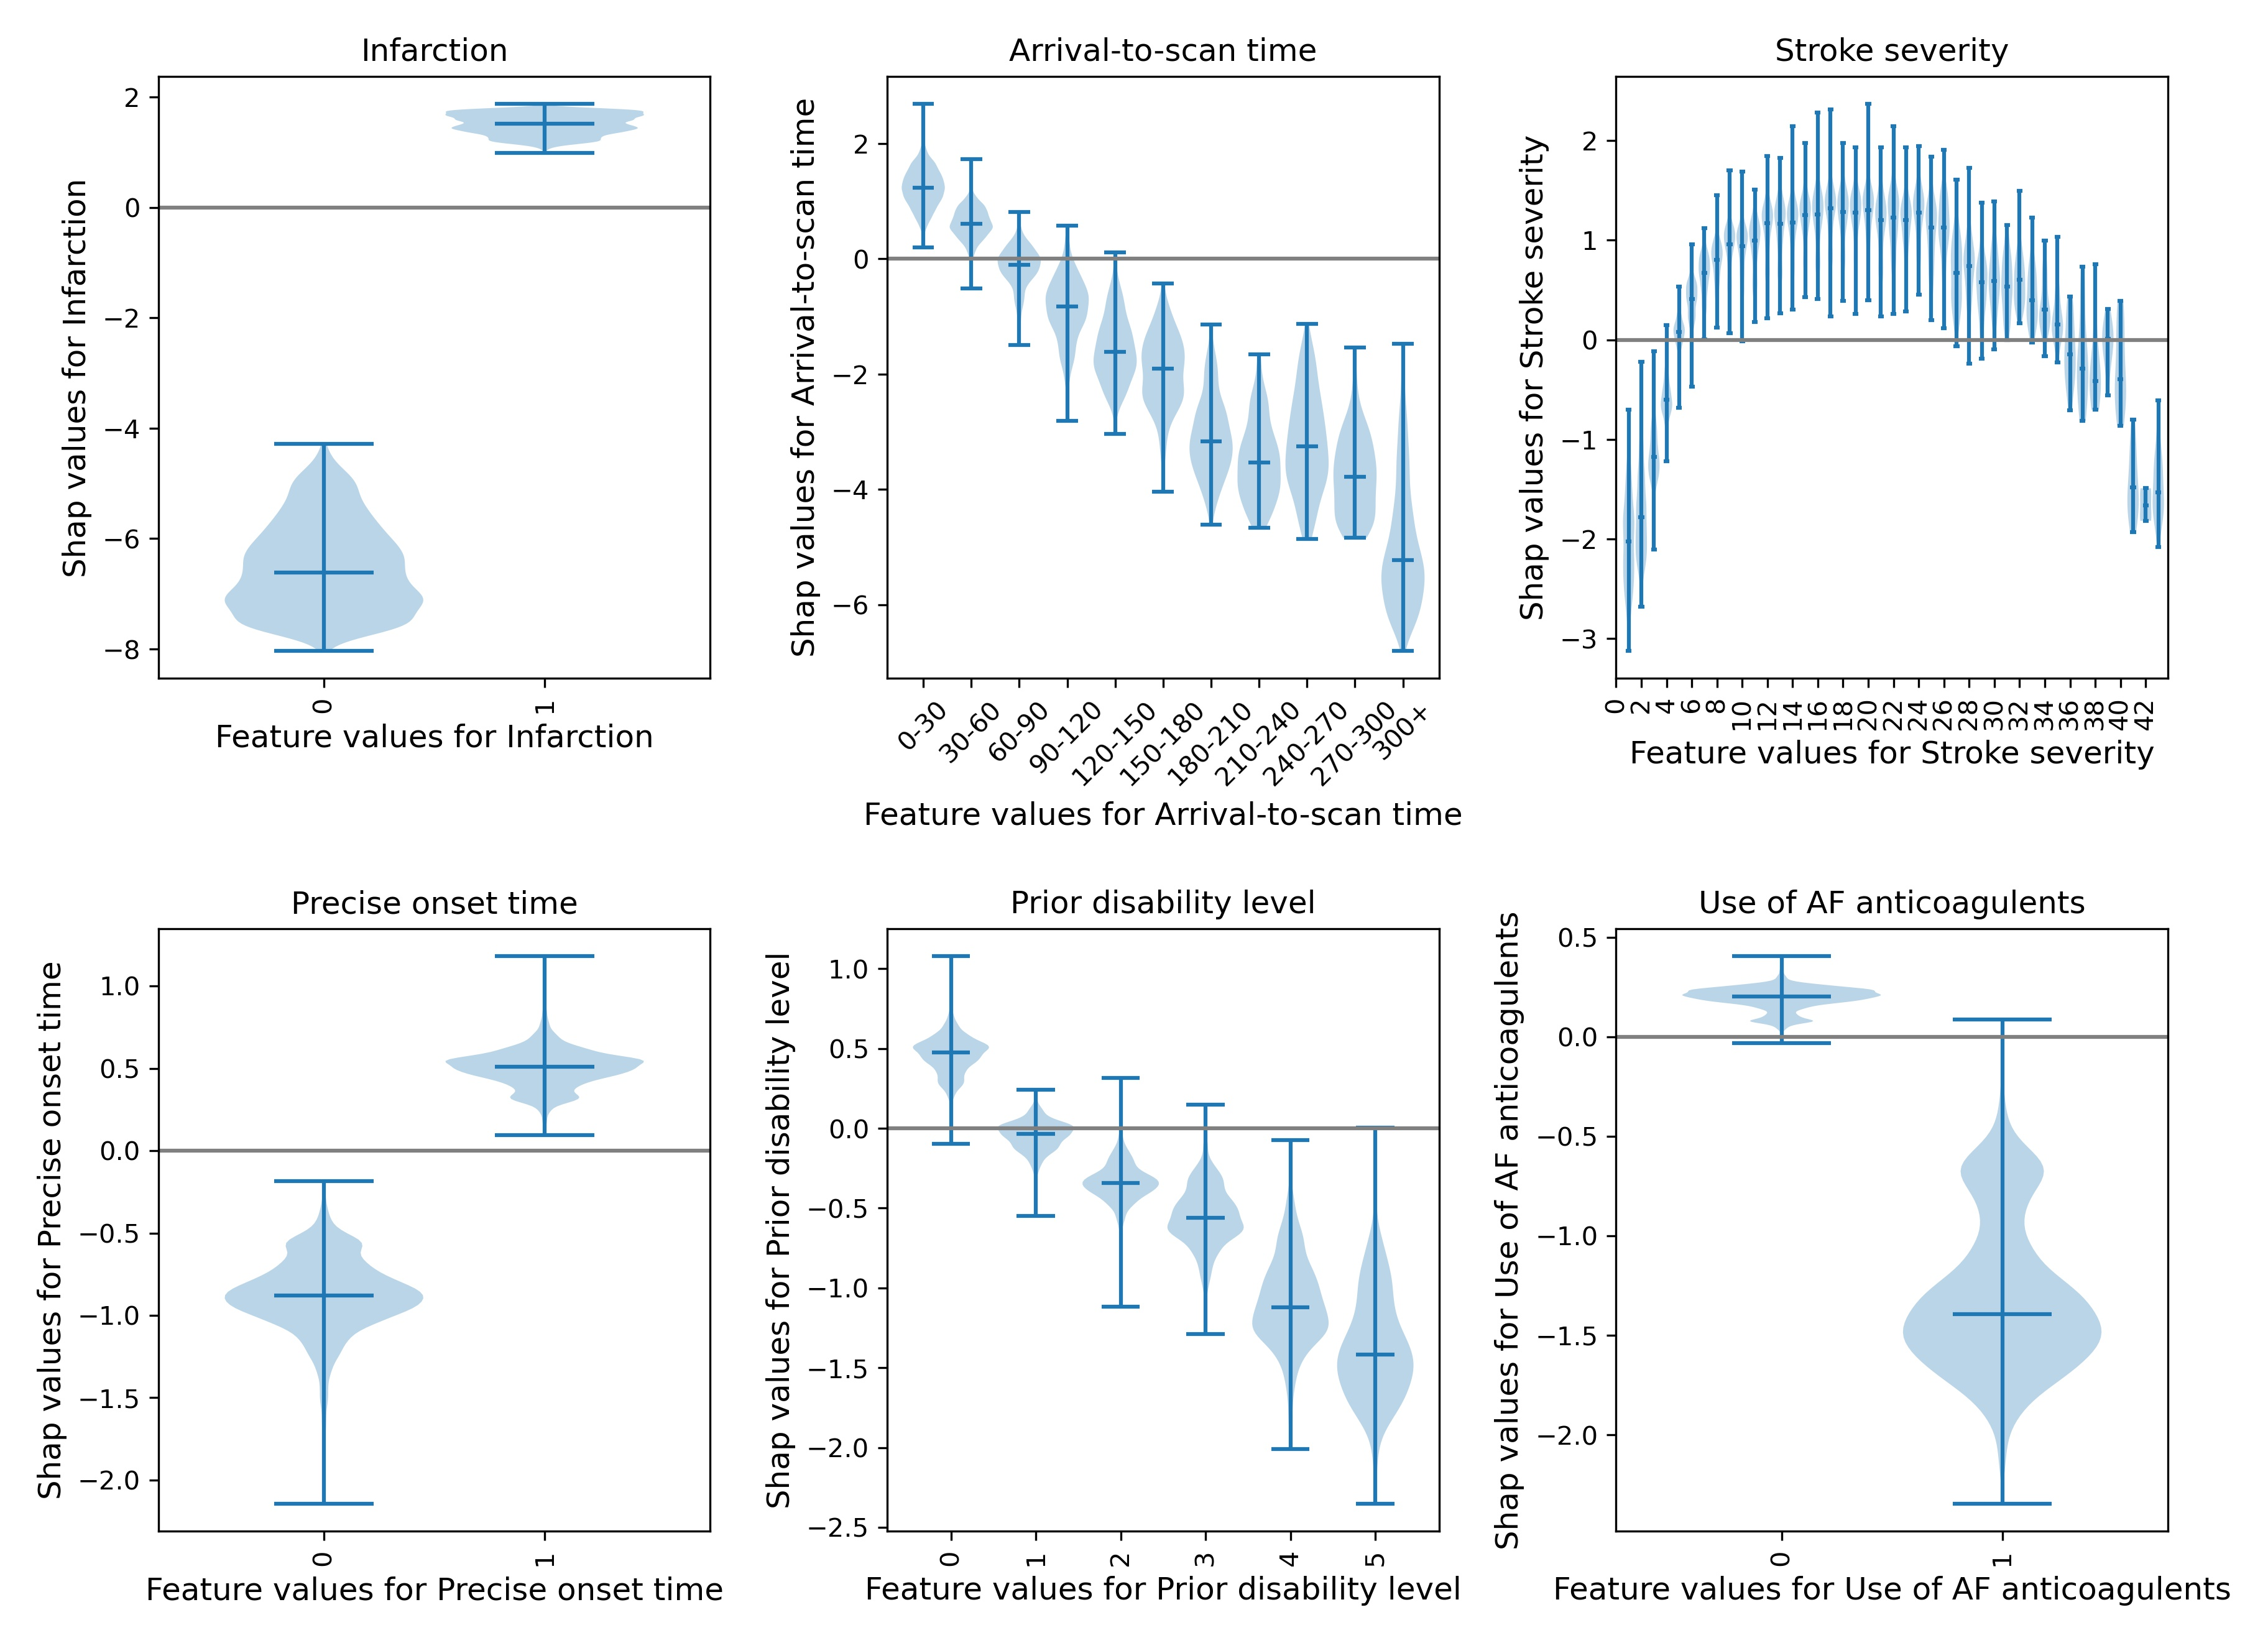
\includegraphics[width=0.80\textwidth]{./images/xgb_thrombolysis_shap_violin.jpg}
\end{center}
\end{frame}

%%%%%%%%%%%%%%%%%%%%%%%%%%%%%%%%%%%%%%%%%%%%%%%%%%%%%%%%%%%%%%%

\begin{frame}
\frametitle{Investigating how hospitals differ in thrombolysis decision-making (Patient 1: Base patient)}

Assuming there are no reasons not stated here to exclude a patient from use of thrombolysis, would you give this patient thrombolysis?
\vspace{3mm}

\begin{columns}
    \begin{column}{0.5\textwidth}
        \begin{itemize}
            \item Onset to arrival = 80 mins
            \item Arrival to scan = 20 mins
            \item Infarction = Yes
            \item NIHSS = 15
            \item Prior disability level = 0
            \item Precise onset time = Yes
            \item Use of AF anticoagulents = No
        \end{itemize}
    \end{column}
    
    \begin{column}{0.4\textwidth}
    Our model predicts 131 out of 132 (99\%) hospitals would give this patient thrombolysis.
    \end{column}

\end{columns}
\end{frame}

%%%%%%%%%%%%%%%%%%%%%%%%%%%%%%%%%%%%%%%%%%%%%%%%%%%%%%%%%%%%%%%

\begin{frame}
\frametitle{Investigating how hospitals differ in thrombolysis decision-making (Patient 2: Milder stroke)}

Assuming there are no reasons not stated here to exclude a patient from use of thrombolysis, would you give this patient thrombolysis?

\vspace{3mm}

\begin{columns}
    \begin{column}{0.5\textwidth}
        \begin{itemize}
            \item Onset to arrival = 80 mins
            \item Arrival to scan = 20 mins
            \item Infarction = Yes
            \item \emph{NIHSS = 4}
            \item Prior disability level = 0
            \item Precise onset time = Yes
            \item Use of AF anticoagulents = No
        \end{itemize}
    \end{column}
    
    \begin{column}{0.4\textwidth}
    Our model predicts 97 out of 132 (73\%) hospitals would give this patient thrombolysis.
    \end{column}

\end{columns}
\end{frame}

%%%%%%%%%%%%%%%%%%%%%%%%%%%%%%%%%%%%%%%%%%%%%%%%%%%%%%%%%%%%%%%

\begin{frame}
\frametitle{Investigating how hospitals differ in thrombolysis decision-making (Patient 3: Pre-stroke disability)}

Assuming there are no reasons not stated here to exclude a patient from use of thrombolysis, would you give this patient thrombolysis?

\vspace{3mm}

\begin{columns}
    \begin{column}{0.5\textwidth}
        \begin{itemize}
            \item Onset to arrival = 80 mins
            \item Arrival to scan = 20 mins
            \item Infarction = Yes
            \item NIHSS = 15
            \item \emph{Prior disability level = 3*}
            \item Precise onset time = Yes
            \item Use of AF anticoagulents = No
        \end{itemize}
    \vspace{3mm}    
    \footnotesize{*Moderate disability; requires some help, but able to walk without assistance.}
    \end{column}
    
    \begin{column}{0.4\textwidth}
    Our model predicts 114 out of 132 (86\%) hospitals would give this patient thrombolysis.
    \end{column}

\end{columns}
\end{frame}

%%%%%%%%%%%%%%%%%%%%%%%%%%%%%%%%%%%%%%%%%%%%%%%%%%%%%%%%%%%%%%%

\begin{frame}
\frametitle{Investigating how hospitals differ in thrombolysis decision-making (Patient 4: Estimated stroke onset time)}

Assuming there are no reasons not stated here to exclude a patient from use of thrombolysis, would you give this patient thrombolysis?

\vspace{3mm}

\begin{columns}
    \begin{column}{0.5\textwidth}
        \begin{itemize}
            \item Onset to arrival = 80 mins
            \item Arrival to scan = 20 mins
            \item Infarction = Yes
            \item NIHSS = 15
            \item Prior disability level = 0
            \item \emph{Precise onset time = No}
            \item Use of AF anticoagulents = No
        \end{itemize}
    \end{column}
    
    \begin{column}{0.4\textwidth}
    Our model predicts 84 out of 132 (64\%) hospitals would give this patient thrombolysis.
    \end{column}

\end{columns}
\end{frame}


%%%%%%%%%%%%%%%%%%%%%%%%%%%%%%%%%%%%%%%%%%%%%%%%%%%%%%%%%%%%%%%
\begin{frame}
\frametitle{Machine Learning key findings}
General observations about thrombolysis use: The chance of receiving thrombolysis is increased by:
\emph{
\begin{itemize}
    \item Shorter arrival-to-scan times
    \item Mid-level stroke severity
    \item Precise onset time
    \item Lower pre-stroke disability
\end{itemize}
}

\vspace{5mm}

Lower thrombolysing units are particularly less likely to give thrombolysis to patients with:
\emph{
\begin{itemize}
    \item Low or high stroke severity
    \item Higher pre-stroke disability
    \item Estimated onset time
\end{itemize}
}

\end{frame}

%%%%%%%%%%%%%%%%%%%%%%%%%%%%%%%%%%%%%%%%%%%%%%%%%%%%%%%%%%%%%%%
%%%%%%%%%%%%%%%%%%%%%%%%%%%%%%%%%%%%%%%%%%%%%%%%%%%%%%%%%%%%%%%
%%%%%%%%%%%%%%%%%%%%%%%%%%%%%%%%%%%%%%%%%%%%%%%%%%%%%%%%%%%%%%%
%%%%%%%%%%%%%%%%%%%%%%%%%%%%%%%%%%%%%%%%%%%%%%%%%%%%%%%%%%%%%%%

%%%%%%%%%%%%%%%%%%%%%%%%%%%%%%%%%%%%%%%%%%%%%%%%%%%%%%%%%%%%%%%
\section{Stroke outcome modelling based on times to treatment with thrombolysis and thrombectomy}



%%%%%%%%%%%%%%%%%%%%%%%%%%%%%%%%%%%%%%%%%%%%%%%%%%%%%%%%%%%%%%%

\begin{frame}{Model combines multiple data sources}

\begin{center}
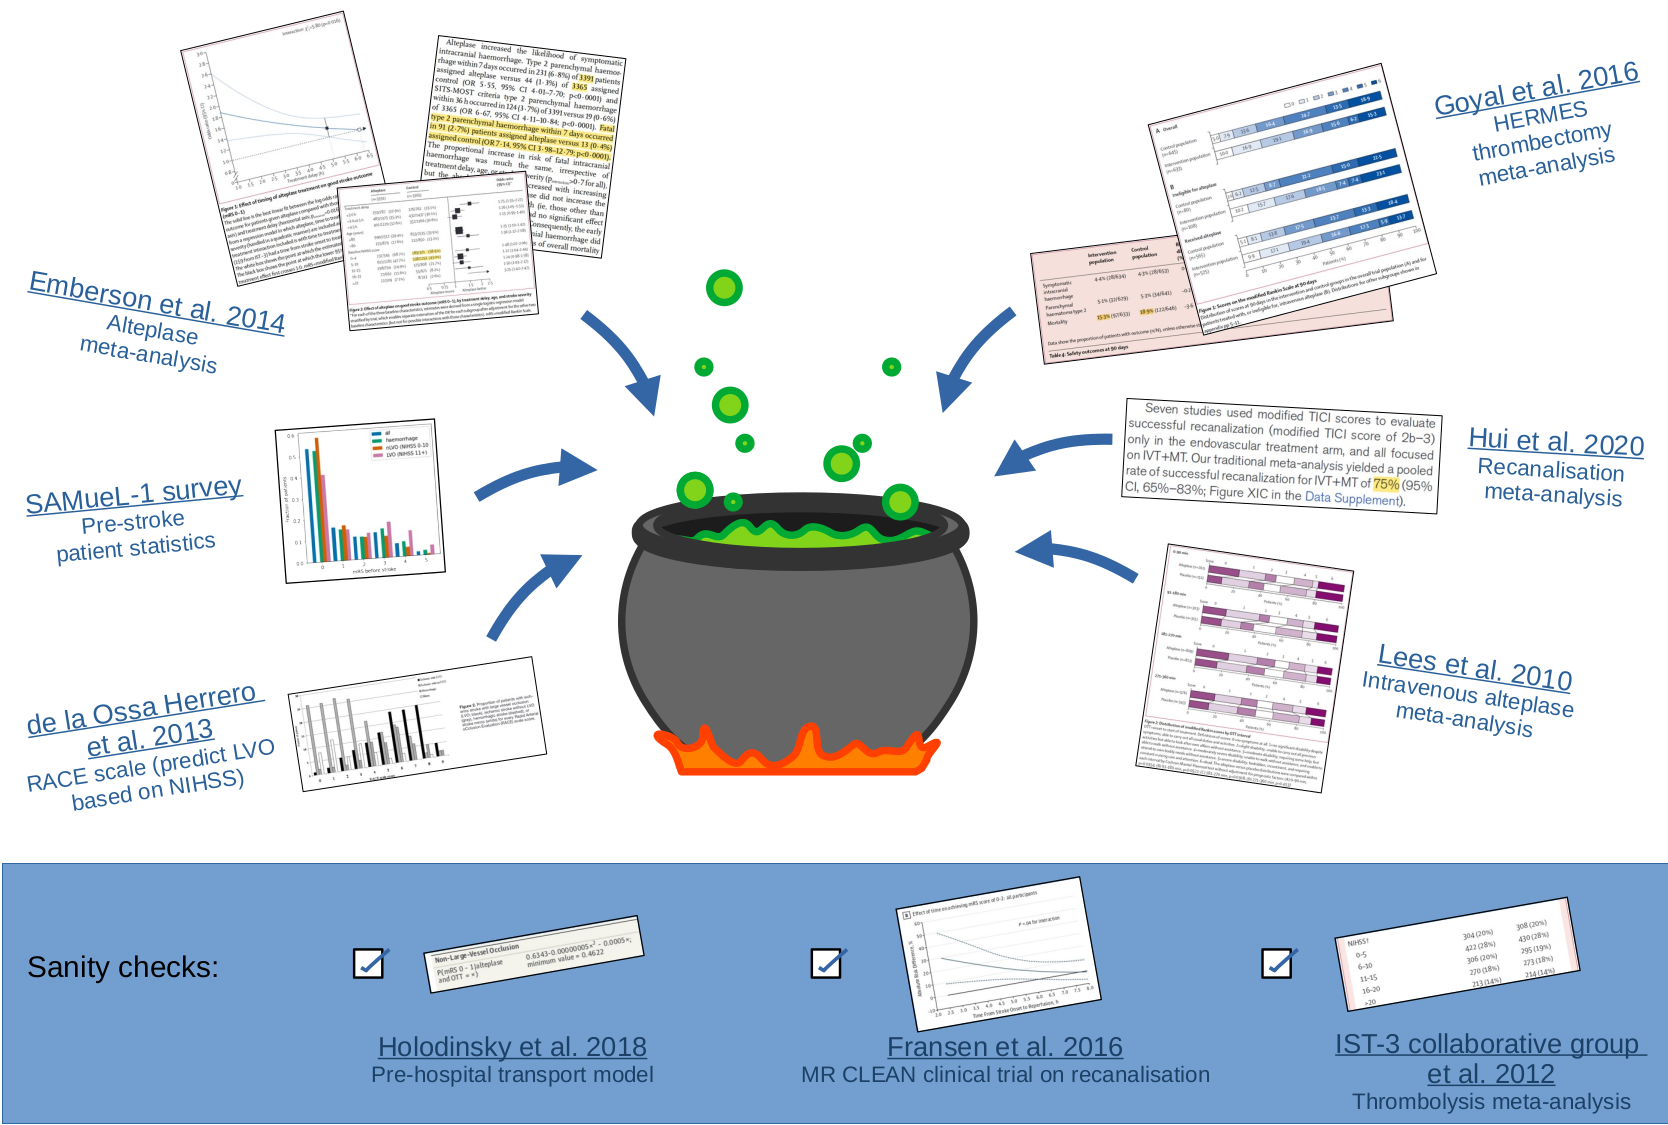
\includegraphics[width=0.90\textwidth]{./images/data_couldron}
\end{center}
    
\end{frame}

%%%%%%%%%%%%%%%%%%%%%%%%%%%%%%%%%%%%%%%%%%%%%%%%%%%%%%%%%%%%%%%

\begin{frame}{Prediction of mRS-level outcomes based on time to treatment}

\begin{center}
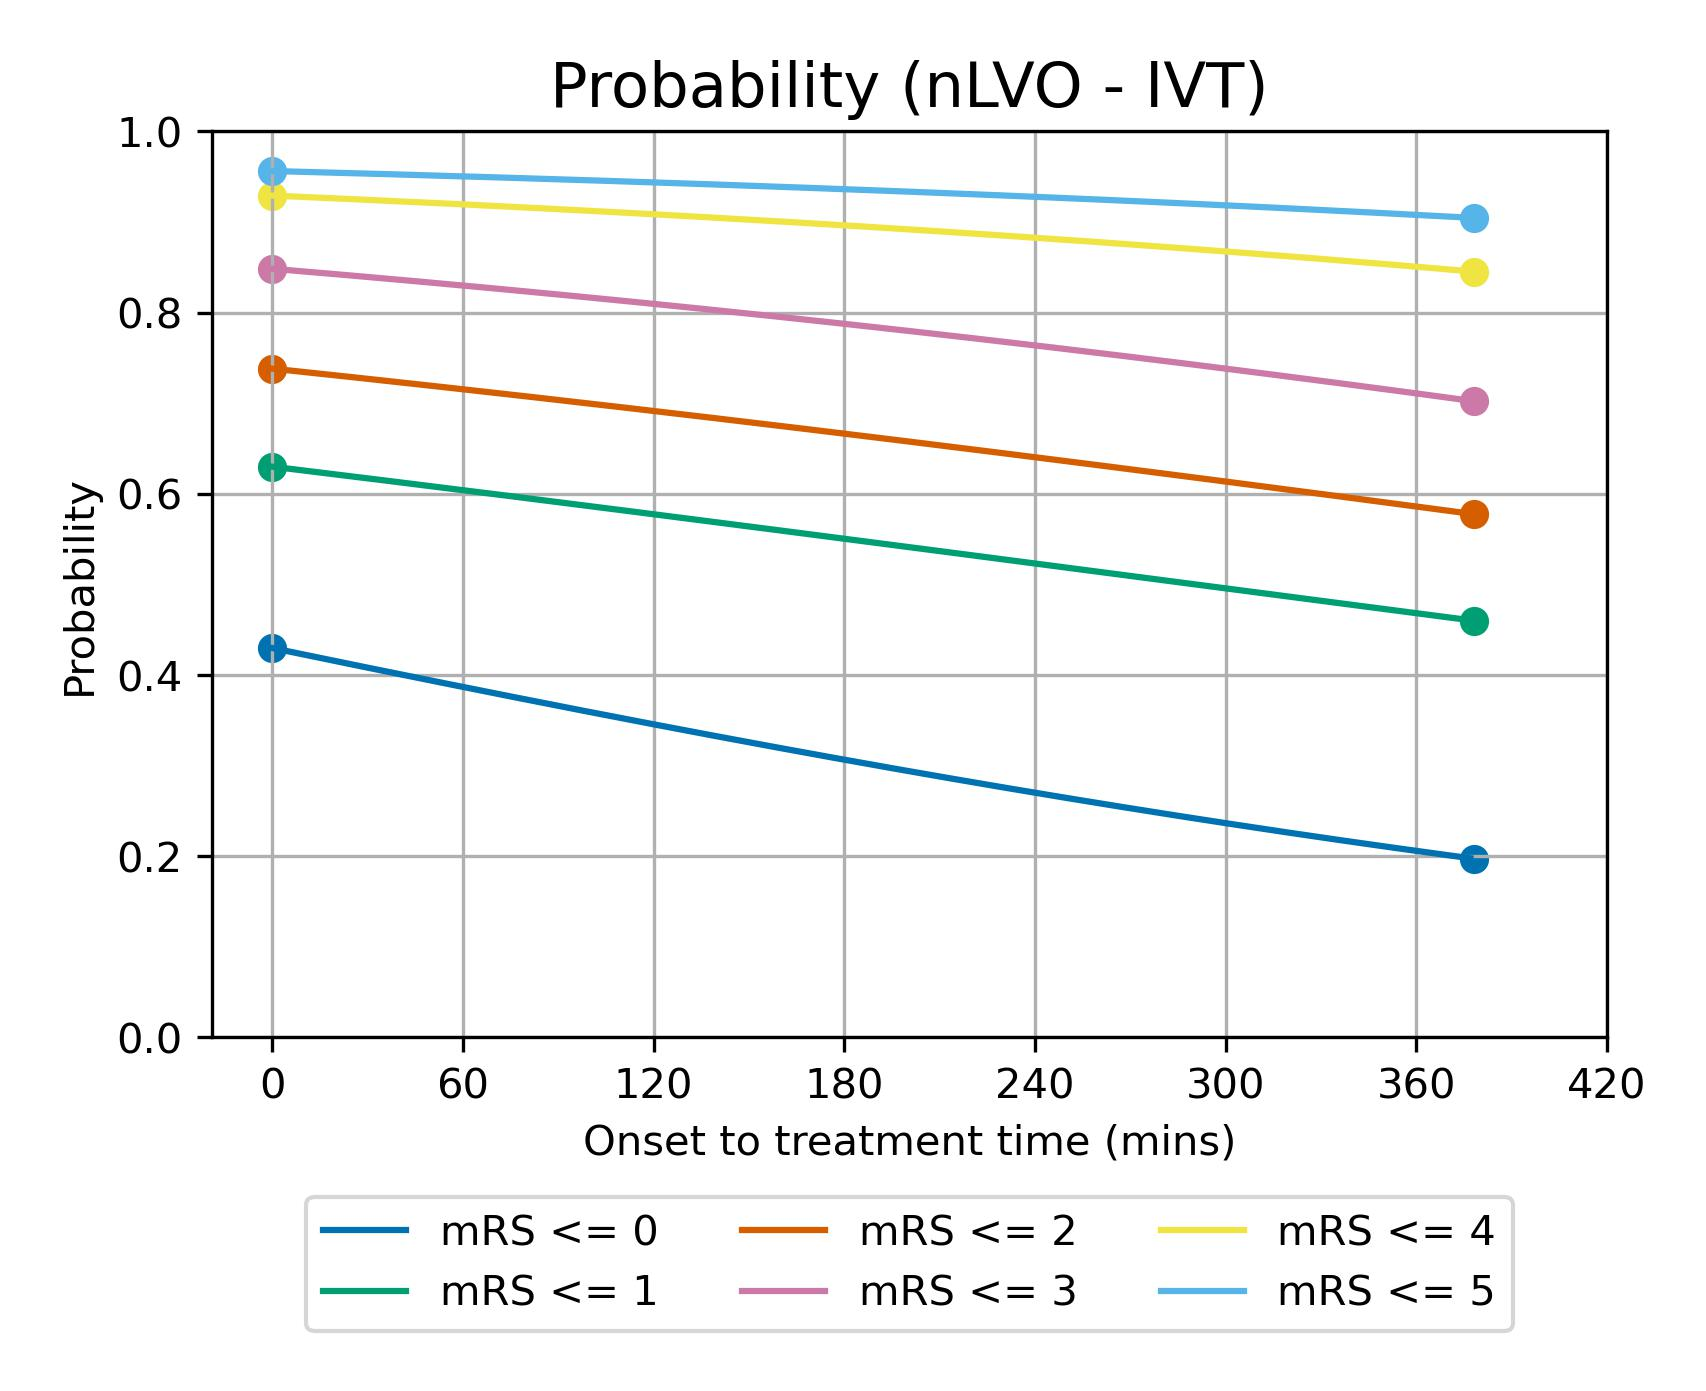
\includegraphics[width=0.80\textwidth]{./images/prob_with_time_nlvo_ivt}
\end{center}
    
\end{frame}

%%%%%%%%%%%%%%%%%%%%%%%%%%%%%%%%%%%%%%%%%%%%%%%%%%%%%%%%%%%%%%%

\begin{frame}{Summary of benefit and added utility by stroke type and treatment type}

\begin{center}
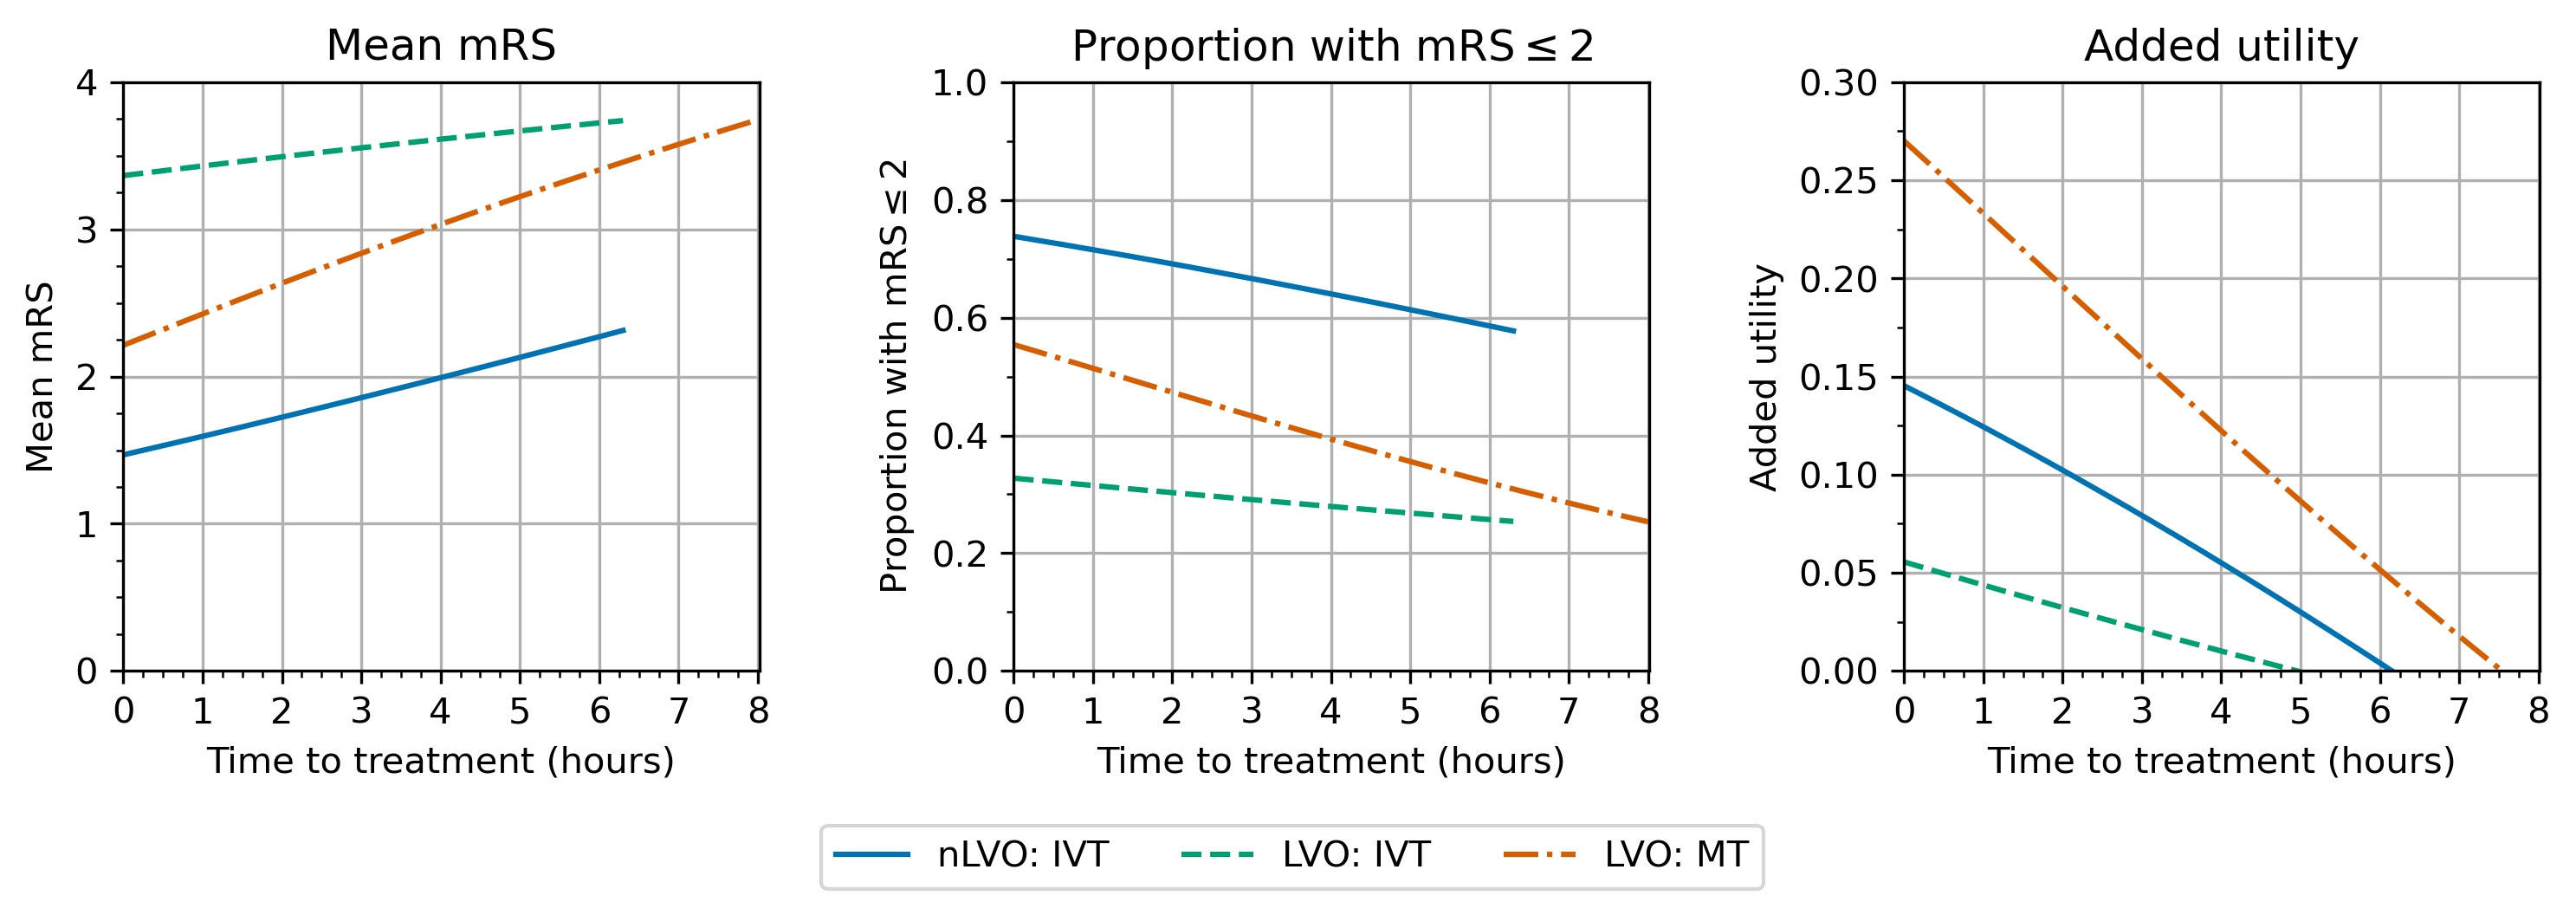
\includegraphics[width=1.0\textwidth]{./images/time_to_treatment}
\end{center}
    
\end{frame}

%%%%%%%%%%%%%%%%%%%%%%%%%%%%%%%%%%%%%%%%%%%%%%%%%%%%%%%%%%%%%%%
\section{HQIP data request}

\begin{frame}{HQIP data request}

\begin{itemize}
    \setlength\itemsep{3mm}
    \item Request for new data has been submitted to HQIP
    \item New data will de-anonymize hospitals, and include ambulance times
    \item Knowledge of hospital will allow linkage to SSNAP organisational audit data
    \item We had informal input from HQIP, and agreement that our data request can be considered as anonymised data, but there remains a small risk that HQIP will not consider data sufficiently anonymised.
\end{itemize}
    
\end{frame}

%%%%%%%%%%%%%%%%%%%%%%%%%%%%%%%%%%%%%%%%%%%%%%%%%%%%%%%%%%%%%%%
\section{Qualitative research}



\begin{frame}{Qualitative research key themes}

\emph{"Finding out what does it take to get AI stuff USEFULLY incorporated [adopted] into a national audit"}

\vspace{5mm}

Qualitative research has been reviewed, and we are now proposing three components:
\vspace{2mm}

\begin{itemize}
    \item Observation case studies
    \item Interviews (individual and group)
    \item Model and AI development stakeholder meetings
\end{itemize}

\end{frame}
%%%%%%%%%%%%%%%%%%%%%%%%%%%%%%%%%%%%%%%%%%%%%%%%%%%%%%%%%%%%%%%

\begin{frame}{Observation case studies}

\begin{itemize}
    \setlength\itemsep{3mm}
    \item 2 weeks each at three hospitals
    \item Observation of emergency stroke care
    \item Interviews about SAMueL analysis for that hospital
    \item If possible, a (virtual) stakeholder workshop at each hospital, with modellers
\end{itemize}
\end{frame}



%%%%%%%%%%%%%%%%%%%%%%%%%%%%%%%%%%%%%%%%%%%%%%%%%%%%%%%%%%%%%%%

\begin{frame}{Interviews (individual and group)}

\begin{itemize}
    \setlength\itemsep{3mm}
    \item Broaden input to wider than three main case study hospitals
\end{itemize}
\end{frame}

%%%%%%%%%%%%%%%%%%%%%%%%%%%%%%%%%%%%%%%%%%%%%%%%%%%%%%%%%%%%%%%

\begin{frame}{Model and AI development stakeholder meetings}

Engage stakeholders with SAMueL analysis, seek feedback, and refine models and presentation.

\vspace{3mm}

This may occur outside of formal qualitative research.

\vspace{3mm}
Stakeholders include:

\begin{itemize}
    \item Individual hospitals (stroke teams)
    \item Integrated Stroke Delivery Networks
    \item NHS-E Communities of Practice
    \item \emph{Key Informers}, e.g. you!, Sally Evans (NHS-E National Stroke Programme Clinical Policy Unit)
\end{itemize}

\end{frame}

%%%%%%%%%%%%%%%%%%%%%%%%%%%%%%%%%%%%%%%%%%%%%%%%%%%%%%%%%%%%%%%
\begin{frame}{Timelines}

\begin{itemize}
    \setlength\itemsep{4mm}
    \item Qualitative work was delayed by time taken to recruit, and by re-assessment of qualitative plans.
    \item HRA submission now due January 9\textsuperscript{th}. 
    \item Active research to start April.
    \item Work depends on approval by HRA REC \emph{and} NIHR (approval of amendment to protocol). We believe risk of rejection by NIHR is low as we are providing some more in-depth research at no requested extension to project timelines and cost.

\end{itemize}
    
\end{frame}

%%%%%%%%%%%%%%%%%%%%%%%%%%%%%%%%%%%%%%%%%%%%%%%%%%%%%%%%%%%%%%%

\section{Further project materials}

\begin{frame}{Further project materials}

\begin{itemize}
    \setlength\itemsep{4mm}
    \item Key project documents: \url{https://github.com/samuel-book/samuel-2-reference}
    \item SHAP work: \url{https://samuel-book.github.io/samuel_shap_paper_1/}
    \item Stroke outcome modelling: \url{https://samuel-book.github.io/stroke_outcome/}
    
\end{itemize}
    
\end{frame}

%%%%%%%%%%%%%%%%%%%%%%%%%%%%%%%%%%%%%%%%%%%%%%%%%%%%%%%%%%%%%%%

% EXTRA SLIDE(S)

\begin{frame}{}
\end{frame}

\begin{frame}{Reserve slides}
\end{frame}

%%%%%%%%%%%%%%%%%%%%%%%%%%%%%%%%%%%%%%%%%%%%%%%%%%%%%%%%%%%%%%%%%

\begin{frame}
\frametitle{When will low thrombolysing units not use thrombolysis when higher thrombolysing would?}

\footnotesize{Here, a high SHAP shows when a low-thrombolysing unit will reject use of thrombolysis when a higher thrombolysing hospital would use thrombolysis. (Plots are in order of feature importance.)}

\begin{center}
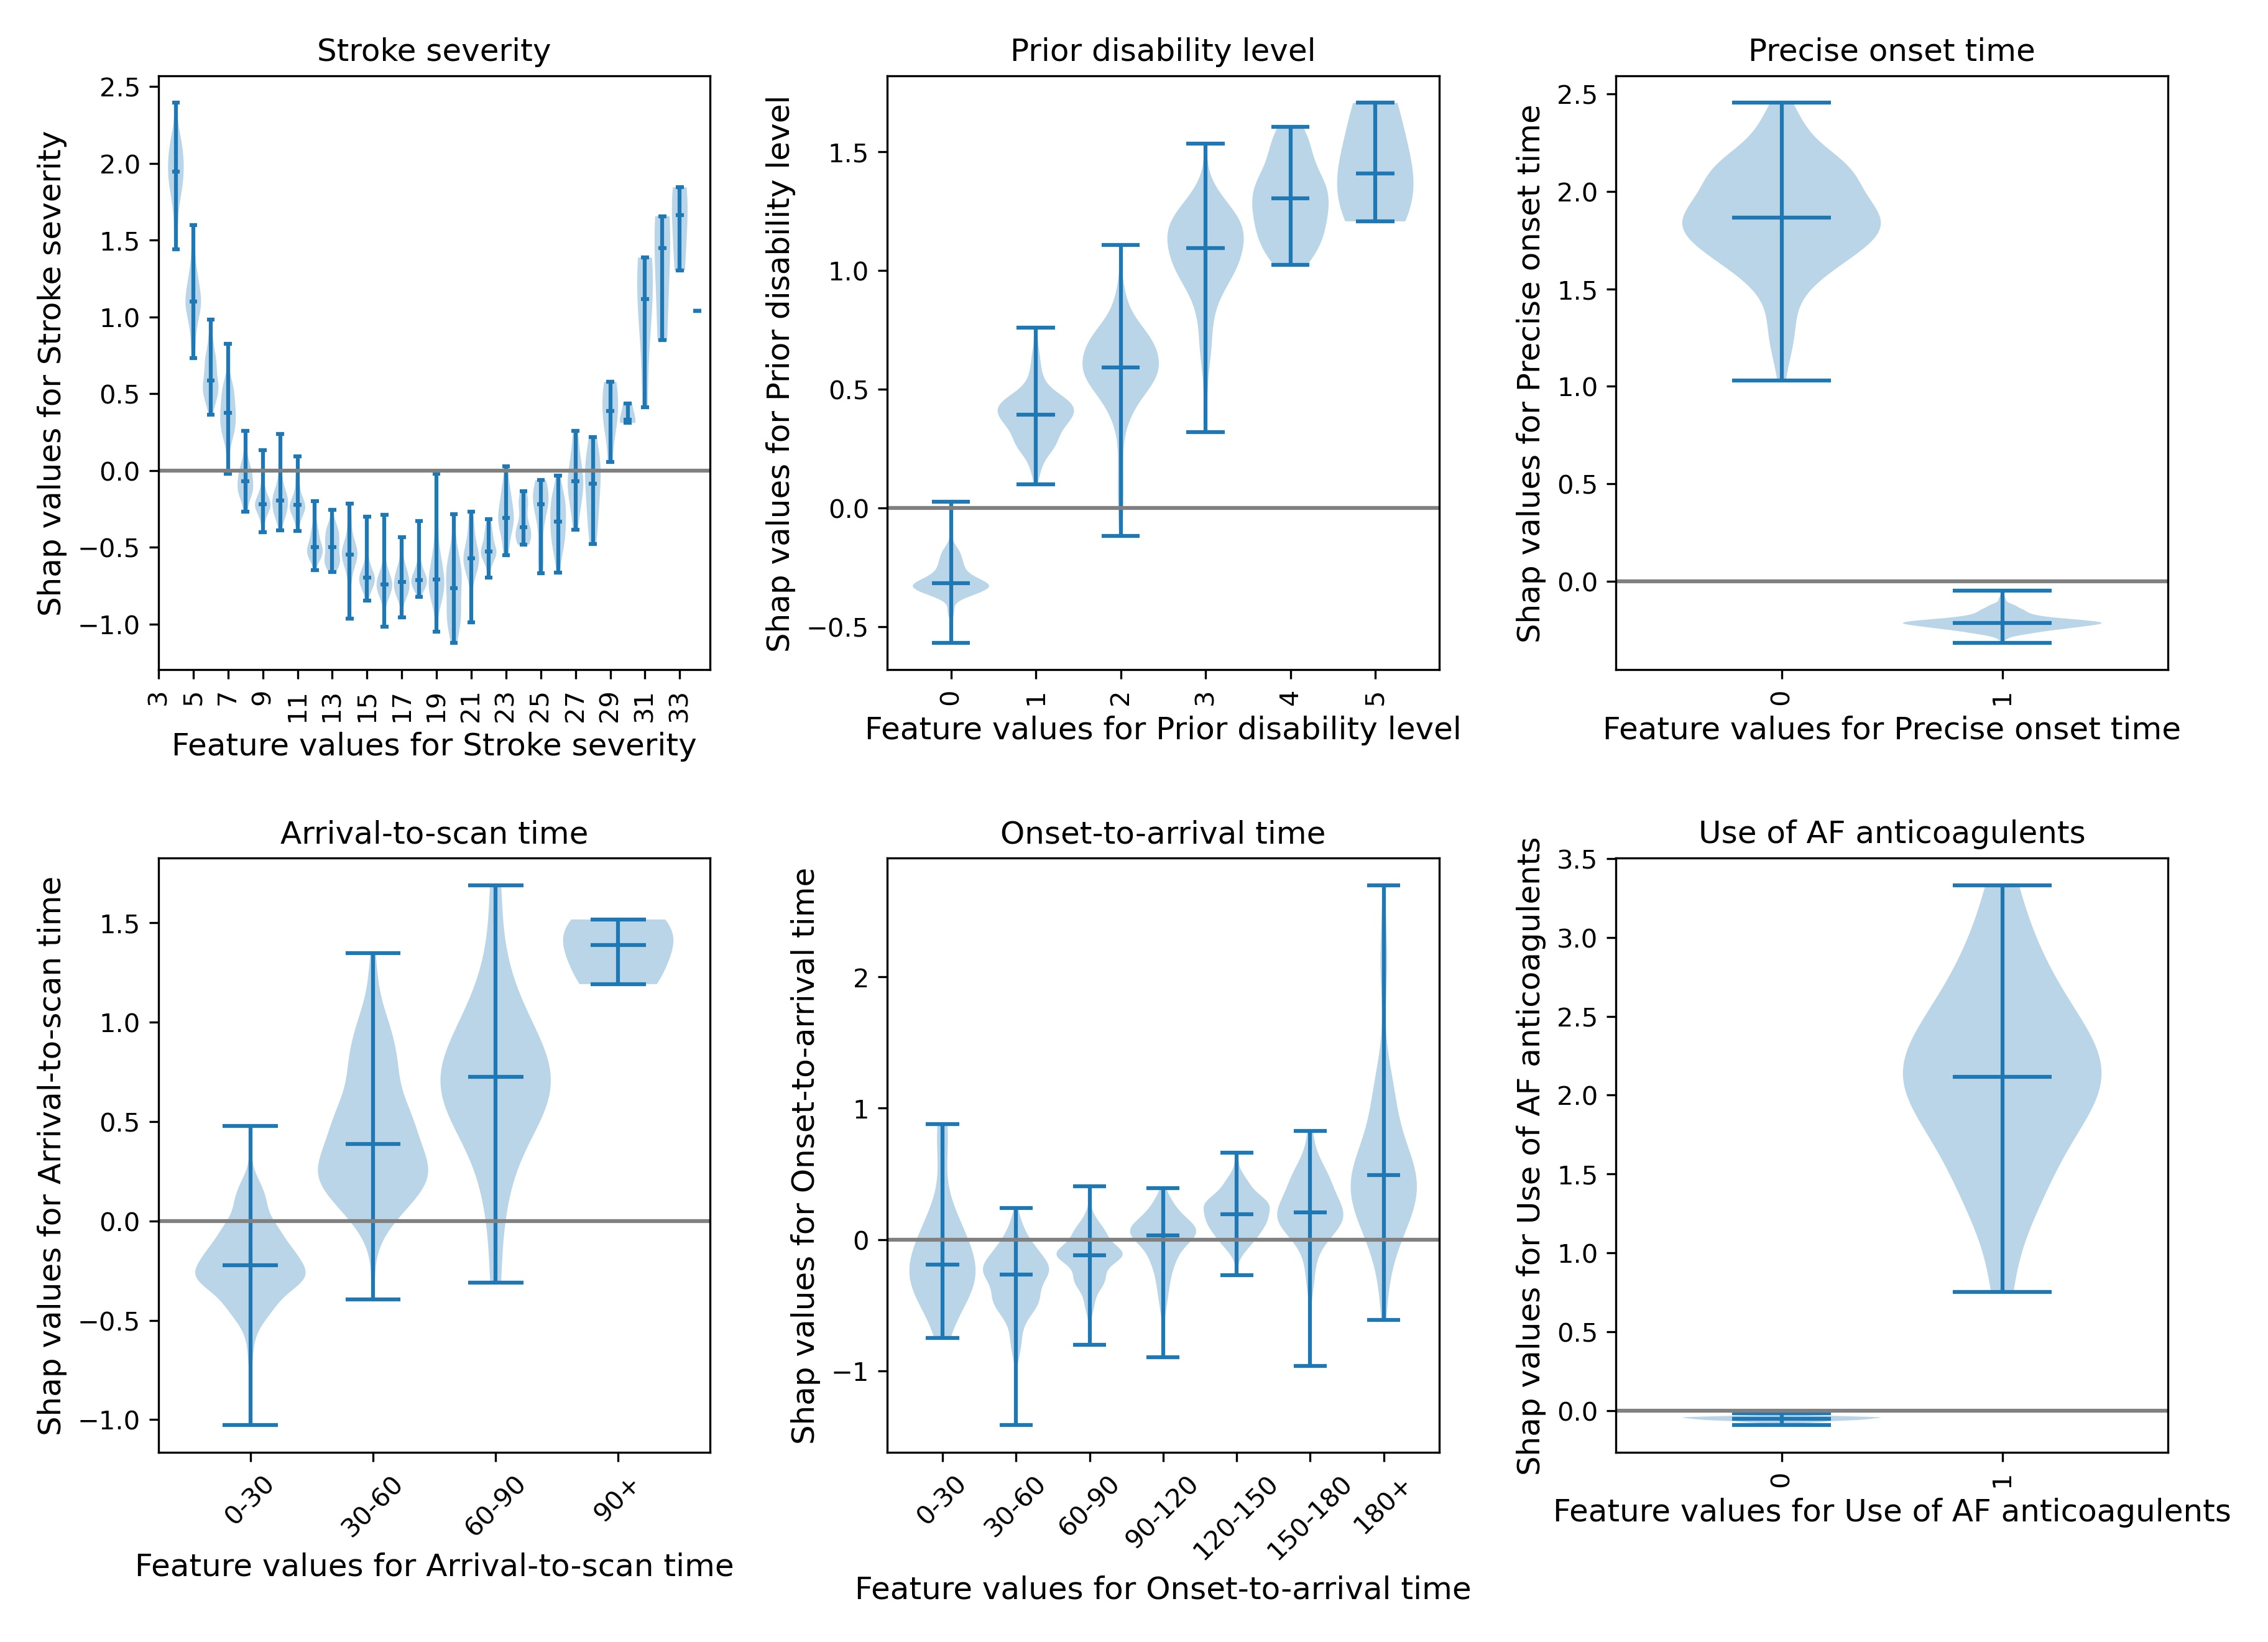
\includegraphics[width=0.75\textwidth]{./images/xgb_predicting_difference_shap_violin.jpg}
\end{center}
\end{frame}



\end{document}




